% English poster. Build: uv run python make_figures.py, then lualatex poster_en.tex twice (the header needs it).
% Shared preamble of poster_en.tex and poster_es.tex (A0 portrait).
\documentclass{article}
\usepackage[paperwidth=841mm,paperheight=1189mm,margin=0mm]{geometry}
\usepackage{fontspec}
\usepackage{unicode-math}
\usepackage[table]{xcolor}
\usepackage{graphicx}
\usepackage{tabularx}
\usepackage{array}
\usepackage{enumitem}
\usepackage{tcolorbox}
\tcbuselibrary{skins}
\usepackage{tikz}
\usetikzlibrary{positioning,arrows.meta,calc}

\setmainfont{Inter_FXH}[Path=C:/Windows/Fonts/, Extension=.ttf, UprightFont=*-Regular, BoldFont=*-Bold,
  ItalicFont=*-Italic, BoldItalicFont=*-BoldItalic]
\setmathfont{Cambria Math}
\setmathfont{Inter_FXH-Regular.ttf}[Path=C:/Windows/Fonts/, range={up/{latin,Latin,num}}]
\setmathfont{Inter_FXH-Italic.ttf}[Path=C:/Windows/Fonts/, range={it/{latin,Latin,greek,Greek}}]

% deep-blue palette with cool neutrals; the same blue marks "this work" in the figures
\definecolor{ink}{HTML}{1A1D24}
\definecolor{muted}{HTML}{5A6170}
\definecolor{rule}{HTML}{D6DAE1}
\definecolor{tile}{HTML}{EEF2F8}
\definecolor{accent}{HTML}{1A4D9C}
\definecolor{accentlight}{HTML}{E6EDF8}
\definecolor{head}{HTML}{0E2550}
\definecolor{headrule}{HTML}{3F72C6}
\definecolor{headmuted}{HTML}{C5D0E3}

% layout: 24 mm side margins, three 251 mm columns with 20 mm gaps
\newlength{\colw}\setlength{\colw}{251mm}
\newlength{\gap}\setlength{\gap}{20mm}
\newlength{\wide}\setlength{\wide}{522mm}
\newlength{\full}\setlength{\full}{793mm}
\newlength{\rowgap}\setlength{\rowgap}{20mm}

\newcommand{\body}{\fontsize{25pt}{32pt}\selectfont\raggedright}
\newcommand{\smalltext}{\fontsize{20pt}{25pt}\selectfont}
\newcommand{\sect}[2]{{\fontsize{38pt}{44pt}\selectfont\bfseries{\color{accent}#1}\hspace{0.45em}#2\par}\vspace{6mm}}
\newcommand{\plainsect}[1]{{\fontsize{38pt}{44pt}\selectfont\bfseries #1\par}\vspace{6mm}}
\newcommand{\sub}[1]{{\fontsize{27pt}{33pt}\selectfont\bfseries #1\par}\vspace{2.5mm}}
\newcommand{\refcite}[1]{{\color{muted}[#1]}}

\setlist[itemize]{label={\color{accent}\rule[0.27em]{0.4em}{0.4em}}, leftmargin=1.1em, itemsep=2.5mm, topsep=1mm,
  parsep=0mm}

% header band: title, subtitle, authors, the paper this work builds on
\newcommand{\posterheader}[4]{%
  \begin{tikzpicture}[remember picture, overlay]
    \fill[head] (current page.north west) rectangle ($(current page.north east) + (0,-142mm)$);
    \fill[headrule] ($(current page.north west) + (0,-142mm)$) rectangle ($(current page.north east) + (0,-145mm)$);
  \end{tikzpicture}%
  \vspace*{22mm}

  \hspace*{24mm}\begin{minipage}[t]{\full}
    \color{white}
    {\fontsize{98pt}{106pt}\selectfont\bfseries #1\par}
    \vspace{7mm}
    {\fontsize{40pt}{48pt}\selectfont\color{headmuted}#2\par}
    \vspace{10mm}
    {\fontsize{30pt}{38pt}\selectfont\bfseries #3\par}
    \vspace{2mm}
    {\fontsize{24pt}{31pt}\selectfont\color{headmuted}#4\par}
  \end{minipage}

  \vspace{40mm}}

% stat tile: big number, what it measures, the paper's value
\newcommand{\stat}[3]{%
  \begin{tcolorbox}[enhanced, colback=tile, colframe=tile, boxrule=0pt, arc=4mm, width=\linewidth,
    left=8mm, right=5mm, top=5mm, bottom=5mm, before skip=0pt, after skip=0pt]
    {\fontsize{58pt}{62pt}\selectfont\bfseries #1\par}\vspace{2.5mm}
    {\fontsize{23pt}{28pt}\selectfont\bfseries #2\par}\vspace{1mm}
    {\fontsize{20pt}{25pt}\selectfont\color{muted}#3\par}
  \end{tcolorbox}}

% HRP repair sketch: a single-linkage dendrogram; #1 duplicate label, #2 held, #3 free
\newcommand{\hrpdiagram}[3]{%
  \begin{tikzpicture}[x=1mm, y=1mm, line width=1.6pt, line cap=round]
    \draw[muted] (0,0)--(0,10)--(22,10)--(22,0);
    \draw[muted] (44,0)--(44,15)--(66,15)--(66,0);
    \draw[muted] (11,10)--(11,28)--(55,28)--(55,15);
    \draw[muted] (88,0)--(88,8)--(110,8)--(110,0);
    \draw[muted] (132,0)--(132,18)--(154,18)--(154,0);
    \draw[muted] (99,8)--(99,23)--(143,23)--(143,18);
    \draw[muted] (33,28)--(33,37)--(121,37)--(121,23);
    \foreach \x/\held in {0/1, 22/0, 44/1, 66/0, 88/0, 110/1, 132/0, 154/1} {
      \ifnum\held=1 \fill[ink] (\x,0) circle (3.2mm);
      \else \filldraw[draw=muted, fill=white, line width=1.5pt] (\x,0) circle (3.2mm); \fi }
    \filldraw[draw=accent, fill=accent] (66,0) circle (3.2mm);
    \draw[accent, line width=2.4pt, -{Stealth[length=5mm, width=4.5mm]}] (46,-5) to[bend right=45] (64,-5);
    \node[font=\smalltext, text=ink, anchor=north] at (55,-13) {#1};
    \fill[ink] (170,22) circle (2.6mm); \node[font=\smalltext, anchor=west, text=muted] at (175,22) {#2};
    \filldraw[draw=muted, fill=white, line width=1.4pt] (170,10) circle (2.6mm);
    \node[font=\smalltext, anchor=west, text=muted] at (175,10) {#3};
  \end{tikzpicture}}

% hybrid loop: #1 genotype, #2 operators, #3 repair, #4 QP, #5 loop label
\newcommand{\pipeline}[5]{%
  \begin{tikzpicture}[x=1mm, y=1mm,
      box/.style={draw=ink, line width=1.5pt, rounded corners=3mm, align=center, minimum height=23mm,
        text width=49mm, font=\fontsize{19pt}{23pt}\selectfont, fill=white, inner xsep=1.5mm},
      arr/.style={-{Stealth[length=4.5mm, width=4mm]}, line width=1.7pt, draw=muted}]
    \node[box] (g) at (0,0) {#1};
    \node[box, right=5mm of g] (v) {#2};
    \node[box, right=5mm of v] (r) {#3};
    \node[box, right=5mm of r, draw=accent, fill=accentlight, line width=2.4pt] (q) {#4};
    \draw[arr] (g) -- (v); \draw[arr] (v) -- (r); \draw[arr] (r) -- (q);
    \draw[arr] (q.south) -- ++(0,-11) -| (g.south);
    \node[font=\smalltext, text=muted, fill=white, inner xsep=3mm] at ($(g.south)!0.5!(q.south) + (0,-11)$) {#5};
  \end{tikzpicture}}

% table rules
\newcommand{\rowrule}{\hline\noalign{\vspace{3mm}}}

\pagestyle{empty}
\setlength{\parindent}{0pt}
\setlength{\parskip}{0pt}


\begin{document}
\color{ink}
\posterheader{Evolve the assets, solve the weights}
  {A hybrid metaheuristic and quadratic programming approach to large-universe portfolio selection}
  {Juan Pedro Enriquez and Eduardo Medina}
  {Replicates and extends Hidalgo-Marín, Nebro \& García-Nieto, \emph{Efficient Selection of Investment Portfolios
  in Real-World Markets}, Algorithms 2026, 19, 20 [1]}

% ------------------------------------------------------------------------------------- row 1
\hspace*{24mm}%
\begin{minipage}[t]{\colw}\body
  \sect{1}{The problem}
  Choose $k$ of $N$ assets and their weights to minimise risk and maximise return:
  \[
    \min\,\bigl(\sigma,-R\bigr),\quad \sigma=\sqrt{250\,w^{\top}\Sigma_S\,w},\quad R=\textstyle\sum_{j\in S} w_j\mu_j
  \]
  \[
    |S|=k,\qquad \textstyle\sum_j w_j=1,\qquad \tfrac{1}{2k}\le w_j\le\tfrac{2}{k}
  \]
  The paper's 12 instances use 2023 daily prices of U.S.-listed assets. The largest, \textbf{ALL\_20\_6000},
  picks $k=20$ of $N=6000$.

  \vspace{9mm}
  \sub{The original study \refcite{1}}
  \begin{itemize}
    \item NSGA-II, MOEA/D, SMS-EMOA and SMPSO (jMetal), 30 runs each.
    \item Real-valued genes: $k$ pointers into the return-sorted asset list and $k$ weights.
    \item SMS-EMOA ranks best. On ALL\_20\_6000 only SMPSO reaches the high-return end.
  \end{itemize}

  \vspace{9mm}
  \sub{Our replica (pymoo)}
  \begin{itemize}
    \item The three evolutionary algorithms with the paper's encoding and settings, 10 runs each.
    \item Same ranking (SMS-EMOA, NSGA-II, MOEA/D) and practically the same fronts: hypervolume 0.944 for both
    on ALL\_20\_6000. Gains below come from the changes, not the framework.
  \end{itemize}
\end{minipage}%
\hspace{\gap}%
\begin{minipage}[t]{\wide}\body
  \sect{2}{What we changed}
  {\fontsize{22pt}{28pt}\selectfont
  \begin{tabularx}{\wide}{@{}>{\bfseries}p{68mm}>{\raggedright\arraybackslash}X>{\raggedright\arraybackslash}X@{}}
    & {\color{muted}\bfseries Original paper [1]} & {\color{accent}\bfseries This work} \\[2mm]
    \arrayrulecolor{rule}\rowrule
    Encoding & $2k$ reals: pointers $s_i\in[0,1]$ pick asset $\lfloor s_i N\rfloor$ of the return-sorted list, plus
      $k$ weights
      & \textbf{Set-based}: $k$ distinct asset IDs, plus one trade-off gene $t\in[0,1]$ \\[3mm]
    \rowrule
    Crossover & SBX on all genes ($p_c=0.9$, $\eta=20$)
      & \textbf{Uniform slot crossover}: each asset comes from either parent \\[3mm]
    \rowrule
    Mutation & Polynomial ($p_m=1/n$, $\eta=20$)
      & \textbf{Swap}: a held asset is exchanged for one outside the portfolio \\[3mm]
    \rowrule
    Duplicates & Next index of the return-sorted list
      & \textbf{HRP repair}: next free leaf of the correlation dendrogram \\[3mm]
    \rowrule
    Weights & Evolved, then normalised and clipped
      & \textbf{Solved exactly} by a QP for the chosen assets \\[3mm]
    \rowrule
    {\mdseries\color{muted}Same} & \multicolumn{2}{>{\raggedright\arraybackslash}p{440mm}}{\color{muted}algorithms,
      settings, evaluation budgets (50\,000--250\,000 per run), seeds, objectives, constraints} \\
  \end{tabularx}\par}

  \vspace{11mm}
  \begin{minipage}[t]{\colw}\raggedright
    \sub{HRP collision repair}
    Slot crossover can give a child the same asset twice. As in Hierarchical Risk Parity \refcite{2}, assets
    are clustered (single linkage) on
    \[ d_{ij}=\sqrt{\tfrac{1}{2}\,(1-\rho_{ij})} \]
    The leaf order puts correlated assets side by side, so a duplicate moves to a close substitute.

    \vspace{6mm}
    \centering
    \hrpdiagram{duplicate $\to$ leaf neighbour}{held}{free}
  \end{minipage}%
  \hspace{\gap}%
  \begin{minipage}[t]{\colw}\raggedright
    \sub{Exact weights: splitting the MIQP}
    The metaheuristic picks the integer part (which assets). What is left is a convex QP in the 20 weights,
    solved exactly for every portfolio (quadprog \refcite{3}):
    \[
      \min_{w}\,\gamma\,\sigma^2-R,\quad \textstyle\sum_j w_j=1,\;\tfrac{1}{2k}\le w_j\le\tfrac{2}{k},\quad
      \gamma=10^{-2+6t}
    \]
    $t$ slides along the efficient frontier of the chosen assets.

    \vspace{6mm}
    \centering
    \pipeline{asset set $S$\\gene $t$}{slot crossover\\swap mutation}{HRP\\repair}{QP weights\\$w^{*}(S,t)$}
      {evaluate $(\sigma,R)$ and select}
  \end{minipage}
\end{minipage}

\vspace{\rowgap}
% ------------------------------------------------------------------------------------- row 2
\hspace*{24mm}\begin{minipage}[t]{\full}\body
  \sect{3}{Results on the largest instance: ALL\_20\_6000}
  \vspace{-2mm}
  {\color{muted}6\,000 assets, $k=20$, 250\,000 evaluations per run. A reference front merges all runs of all
  algorithms: the paper's 4 $\times$ 30 runs, this work's 3 $\times$ 10 runs.\par}
  \vspace{5mm}
  \begin{minipage}[t]{600mm}
    \vspace{0pt}
    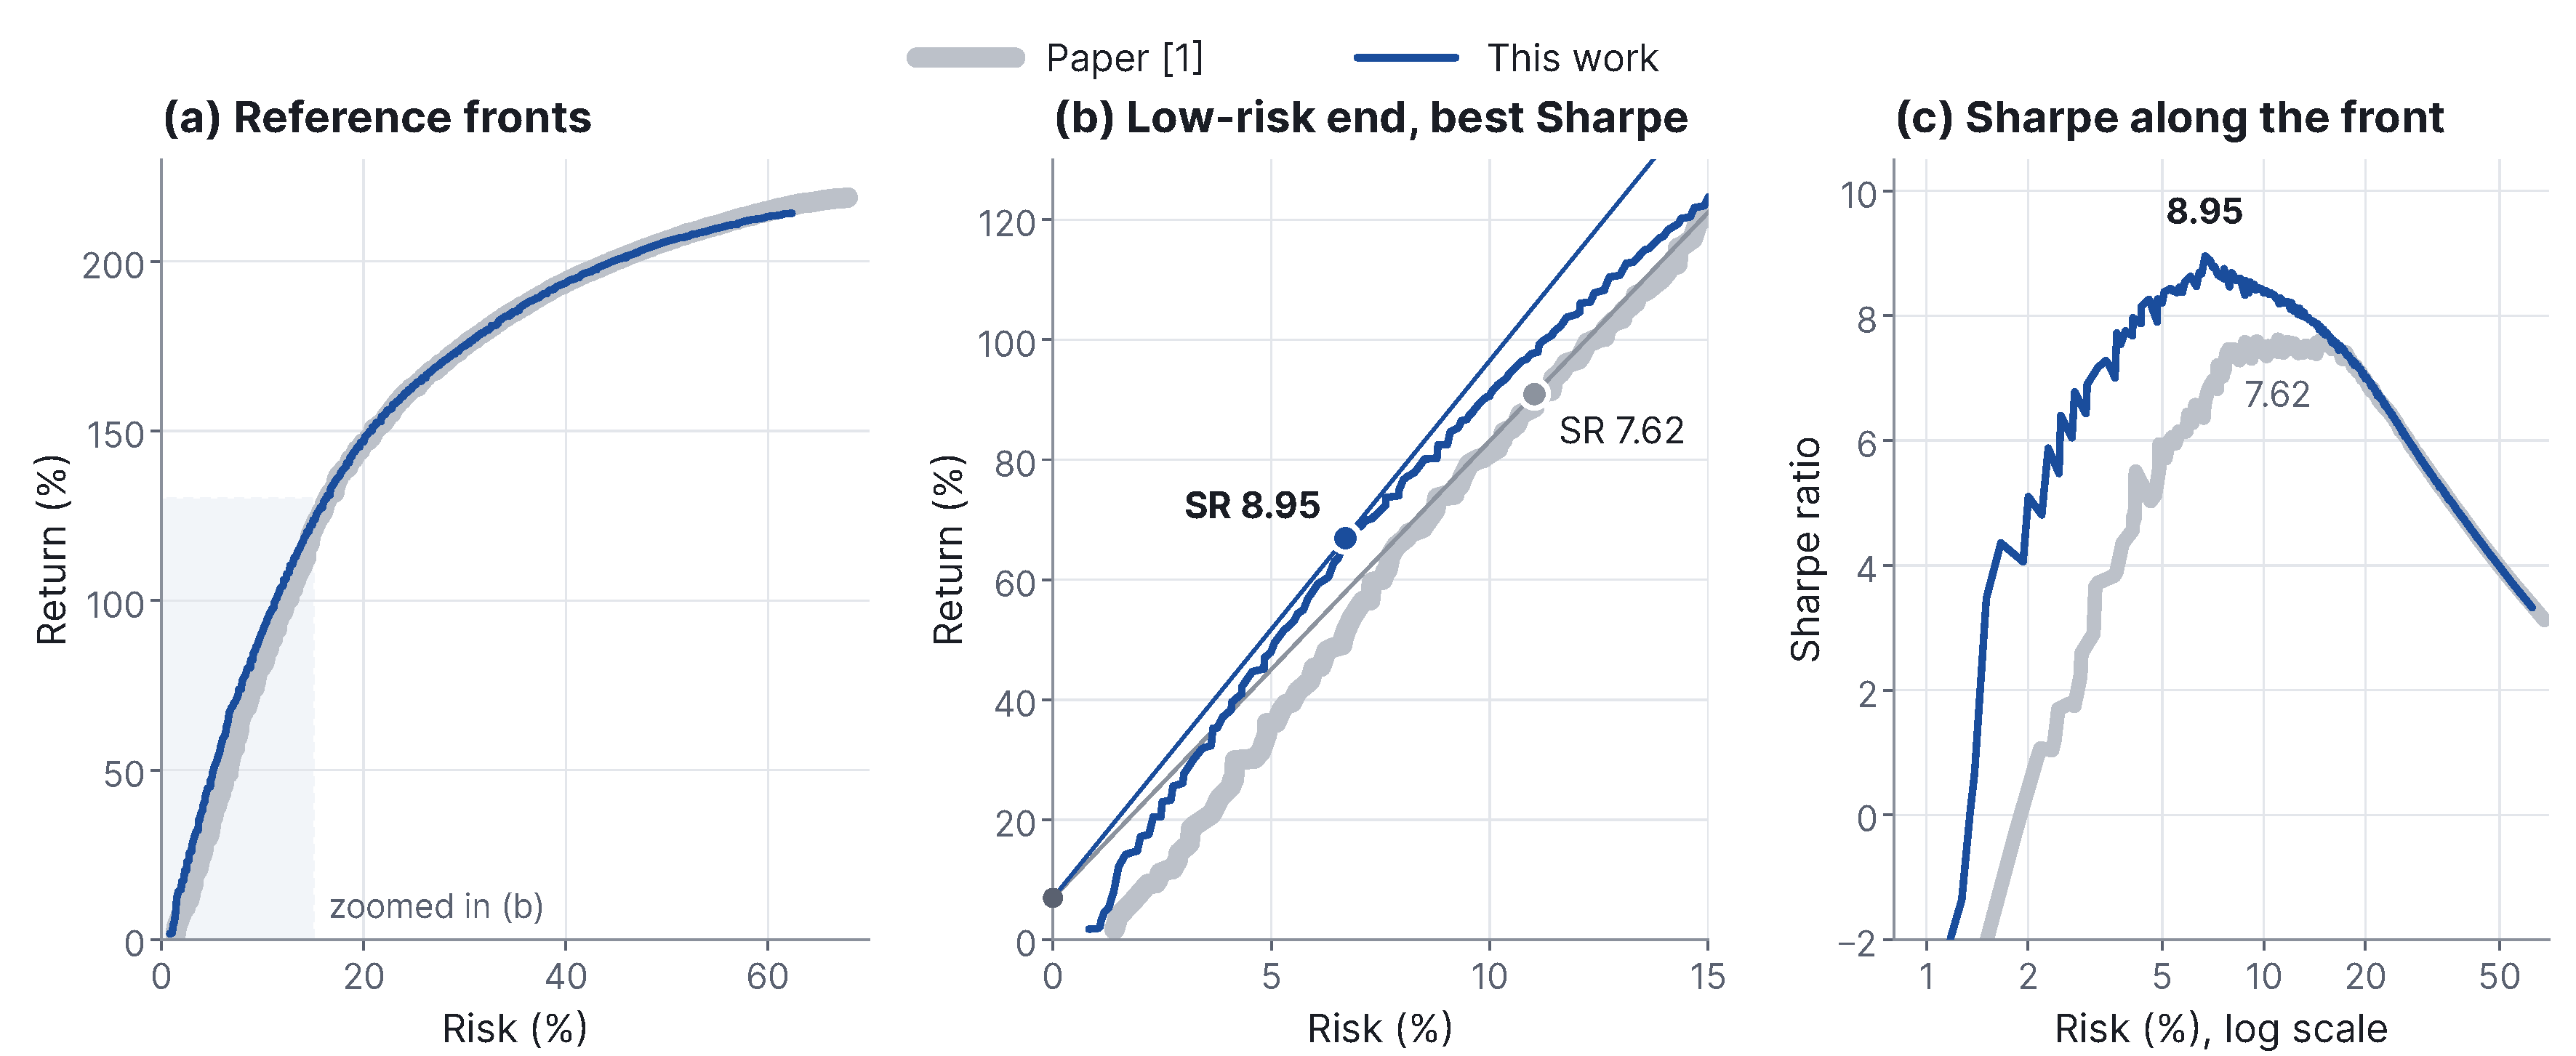
\includegraphics[width=600mm]{figures/fig_all20_6000_en.pdf}\par
    \vspace{2mm}
    {\smalltext\color{muted}(b) The lines from the risk-free rate $R_f=6.97\,\%$ touch each front at its best
    Sharpe ratio $\mathrm{SR}=(R-R_f)/\sigma$, their slope. (c) The Sharpe ratio of every portfolio on each
    front.\par}
  \end{minipage}%
  \hspace{20mm}%
  \begin{minipage}[t]{173mm}
    \vspace{0pt}
    \stat{8.95}{best Sharpe ratio}{paper 7.62 (+18\,\%)}\par\vspace{8mm}
    \stat{+12 pp}{return at 5\,\% risk}{48\,\% vs 36\,\%}\par\vspace{8mm}
    \stat{0.82\,\%}{lowest risk}{paper 1.41\,\%}\par\vspace{8mm}
    \stat{0.951}{hypervolume}{paper 0.944}
  \end{minipage}

  \vspace{8mm}
  The gain sits below 15\,\% risk, where 20 weights are hardest to evolve. Above it the fronts coincide; at the
  top this work reaches 214\,\% return, the paper 219\,\%.
\end{minipage}

\vspace{\rowgap}
% ------------------------------------------------------------------------------------- row 3
\hspace*{24mm}%
\begin{minipage}[t]{\colw}\body
  \sect{4}{Gains grow with $N$}
  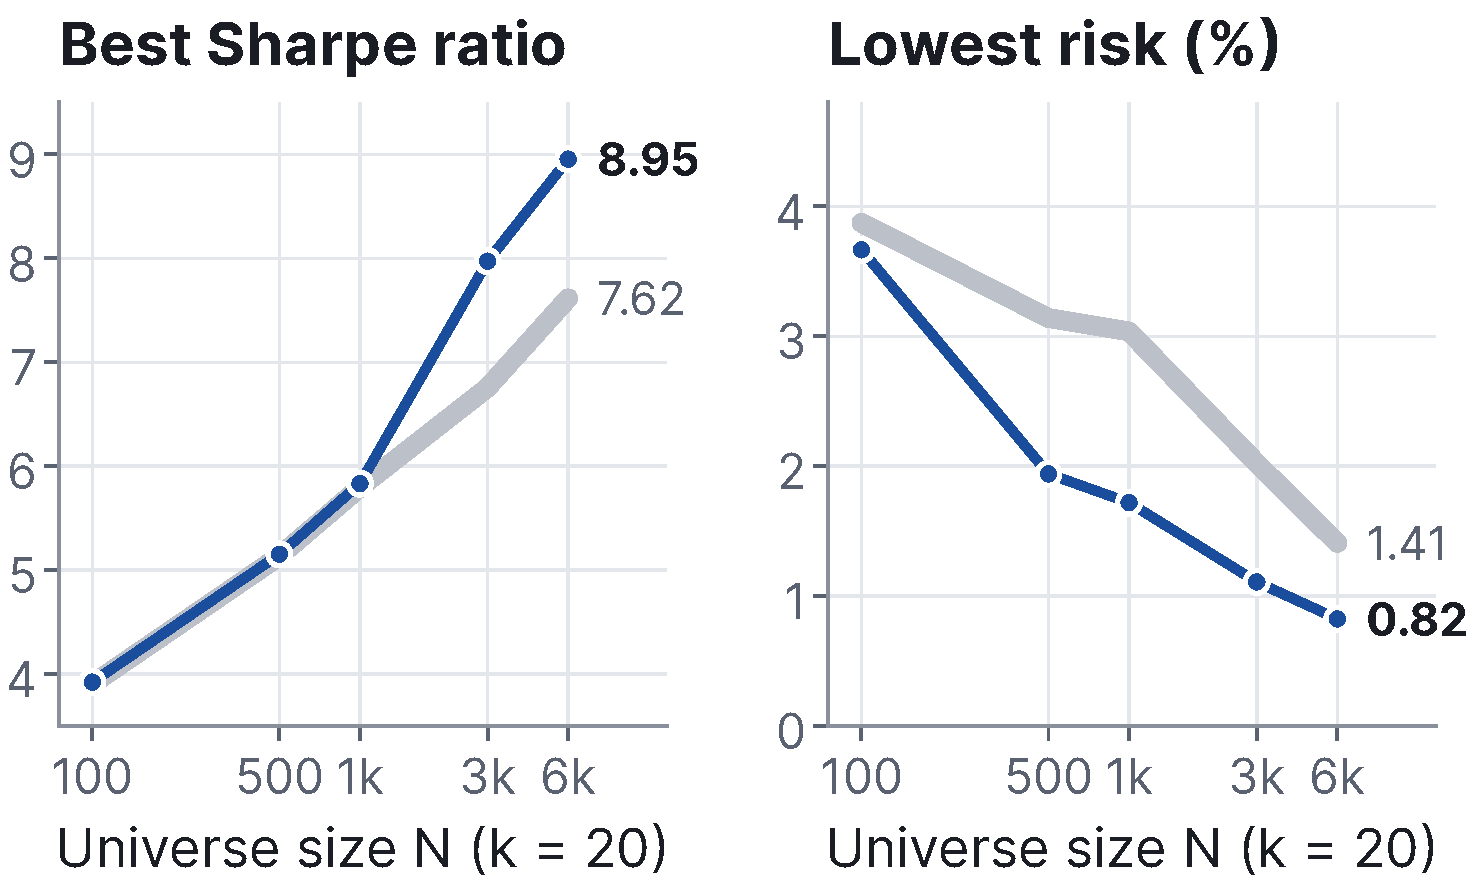
\includegraphics[width=\colw]{figures/fig_scaling_en.pdf}\par
  \vspace{4mm}
  Best hypervolume and IGD+ on all five 20-asset instances; the Sharpe gain jumps at $N\ge 3000$. On the
  5-asset instances the fronts coincide.
\end{minipage}%
\hspace{\gap}%
\begin{minipage}[t]{\colw}\body
  \sect{5}{Robustness and cost}
  \begin{itemize}
    \item \textbf{Per run}, all 12 instances: hypervolume significantly better than the replica's in 33 of 36
    algorithm--instance pairs, never worse (Wilcoxon, 5\,\%). The paper publishes merged fronts only.
    \item \textbf{3 ties}, all on the largest universes (SMS-EMOA on ALL\_20\_3000 and ALL\_20\_6000, NSGA-II
    on ALL\_20\_6000). Single runs there reach lower risk but a shorter high-return end, since swap mutation
    samples 6\,000 assets uniformly.
    \item \textbf{Cost}: same evaluation budget. The QPs raised the time for all 360 runs from 63 to 67 min.
  \end{itemize}
\end{minipage}%
\hspace{\gap}%
\begin{minipage}[t]{\colw}\body
  \sect{6}{Out of sample: 2024}
  Both ALL\_20\_6000 fronts on Yahoo Finance prices: portfolios with 80\,\% of their weight traded in 2023--24,
  leaving out those with a negative Sharpe ratio in both years.

  \vspace{3mm}
  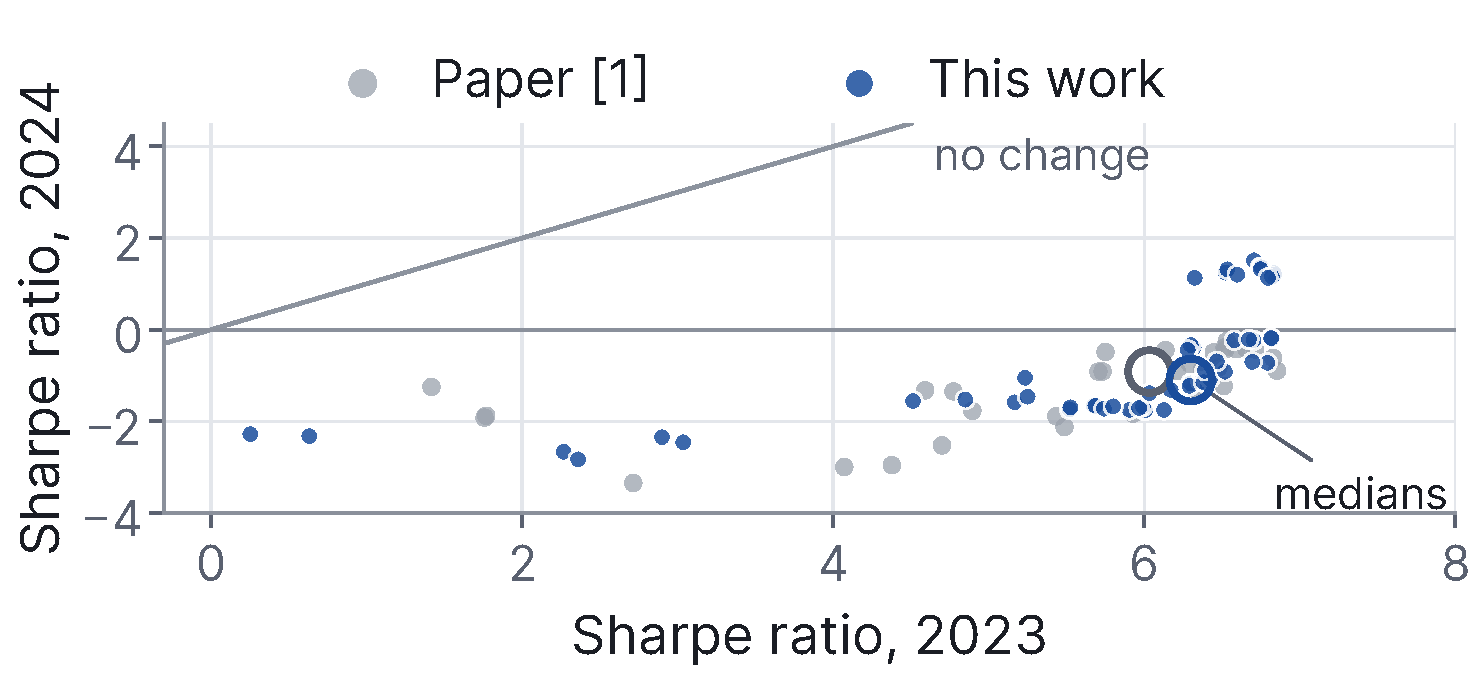
\includegraphics[width=\colw]{figures/fig_oos_en.pdf}\par
  \vspace{3mm}
  Median Sharpe 2023 $\to$ 2024: 6.03 $\to$ $-0.91$ for the paper (32 of 658 portfolios), 6.30 $\to$ $-1.10$
  for this work (54 of 369). The gain is in optimisation, not in forecasting.
\end{minipage}

\vspace{\rowgap}
% ------------------------------------------------------------------------------------- row 4
\hspace*{24mm}%
\begin{minipage}[t]{\wide}\body
  \plainsect{Conclusions}
  \begin{itemize}
    \item A pymoo replica reproduces the paper's ranking and reference fronts.
    \item Evolving only the assets (set encoding, slot crossover, swap mutation, HRP repair) and solving the
    weights by QP gives the best front on every 20-asset instance, and the gain grows with $N$: on
    ALL\_20\_6000 the best Sharpe ratio rises from 7.62 to 8.95 at the same budget.
    \item The gain is in-sample: in 2024 both approaches lose most of their Sharpe ratio. Better estimates of
    returns and risk, rather than a better optimiser, are the next step.
  \end{itemize}
\end{minipage}%
\hspace{\gap}%
\begin{minipage}[t]{\colw}\fontsize{18pt}{23pt}\selectfont\raggedright
  \plainsect{References}
  \vspace{-2mm}
  \begin{enumerate}[label={[\arabic*]}, leftmargin=1.8em, itemsep=2mm, topsep=0mm]
    \item A.\,J. Hidalgo-Marín, A.\,J. Nebro, J. García-Nieto. Efficient Selection of Investment Portfolios in
    Real-World Markets: A Multi-Objective Optimization Approach. \emph{Algorithms} 2026, 19(1), 20.
    doi:10.3390/a19010020
    \item M. López de Prado. Building Diversified Portfolios that Outperform Out of Sample. \emph{J. Portfolio
    Management} 2016, 42(4), 59--69.
    \item D. Goldfarb, A. Idnani. A numerically stable dual method for solving strictly convex quadratic
    programs. \emph{Math. Programming} 1983, 27, 1--33.
    \item J. Blank, K. Deb. pymoo: Multi-Objective Optimization in Python. \emph{IEEE Access} 2020, 8,
    89497--89509.
  \end{enumerate}
\end{minipage}

\end{document}
